Figure \ref{context} is an example of the referential game used in studying human pragmatic inference \cite{Frank}. In a referential game there is a set of objects called the \emph{context}. The speaker in the game is asked to refer to one of the objects (the \emph{target}) by uttering an expression (typically a word) to the listener. The listener, who has no idea which object is the target, needs to recover the speaker's intended referent based on the speaker's utterance. 

\begin{figure}[h] 
  \centering
  \subfigure[The context]{\label{context}
  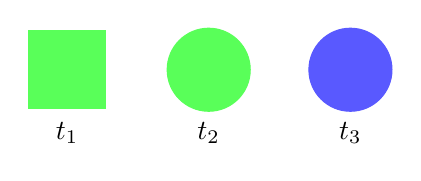
\begin{tikzpicture}
     \path (-1.8, 0) node [shape=rectangle, draw=green!65 ,fill= green!65 ,minimum size=28]{}
           ( 0, 0) node  [shape=circle, draw=green!65, fill= green!65,minimum size=30] {}
           ( 1.8, 0) node [shape=circle, draw=blue!65, fill=blue!65  ,minimum size=30] {}
           ( -1.8, -0.8) node {$t_{1}$}
           ( -0.0, -0.8) node {$t_{2}$}
           (  1.8, -0.8) node {$t_{3}$}
     ;
           
  \end{tikzpicture}
  }  
  \hspace{5mm}
  \subfigure[The vocabulary and the truth table]{\label{VaTT}
  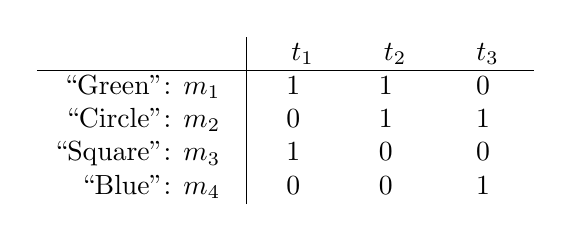
\begin{tikzpicture}
     \path (0,0) node[] 
     {\begin{tabular}{r|ccc}
                         & \quad $t_{1}$\ \  &\quad $t_{2}$\ \  &\quad $t_{3}$ \ \   \\
    \hline
   ``Green'':  $m_{1}$ \quad  &  $1$        &   $1$       & $0$      \\
   ``Circle'': $m_{2}$  \quad &  $0$        &   $1$       & $1$      \\ 
   ``Square'': $m_3$ \quad    &  $1$      &   $0$       & $0$      \\
   ``Blue'':   $m_4$  \quad  &  $0$        &   $0$       & $1$     
     \end{tabular}
     } ;
  \end{tikzpicture}
  }
  \caption{A simple referential game}
\end{figure}


Let us first try to play this game ourselves, to get a better sense of what it is about and why it is relevant to human pragmatic reasoning. For simplicity let us assume that the utterances that the speaker is allowed to use are from a \emph{vocabulary} which is commonly known between the speaker and the listener. The content of the vocabulary and the (truth-conditional/literal) meaning of each word are shown in Figure \ref{VaTT}. Suppose we play as the speaker and the target is $t_1$, the green square. We can either use ``Square'' or ``Green'' to literally truthfully refer to it, but it seems more prudent to use ``Square'', as there is only one square in the context and thus the listener can easily identify it, whereas there are two green objects, which makes ``Green'' ambiguous. In terms of the Gricean \emph{Maxim of Quantity}, we should use ``Square'' because it is as maximally informative as is required. Similarly, we should use ``Blue'' to refer to $t_3$, the blue circle. However,  using ``Blue'' to refer to the blue circle might intuitively sound a little unnatural, as color terms are usually used as adjectives\footnote{They are used as nouns mostly to refer to the colors themselves.}, while we usually use nouns to refer to concrete objects. This inclination becomes more evident when we want to refer to $t_2$, the green circle. While ``Green'' and ``Circle'' are equally ambiguous in this case, we might nevertheless prefer the latter. 

Now let us turn to play as the listener. If we hear ``Square'' or ``Blue'', we easily know the intended referent as there is no ambiguity, but what if we hear ``Circle'' (or ``Green'')? There are two circles in the context that we need to choose from. On the one hand, the blue circle, having the unique color in the context, seems to be perceptually dominant and thus easily captures our attention. On the other hand, from the previous analysis we know that if the blue circle were the intended referent, the speaker could have chosen ``Blue'' which is not ambiguous and thus more informative. Hence the listener needs to balance two sources of information, i.e. the (presumably subconscious) perceptual salience of different objects and the rational expectation of the likelihood of the speaker making the utterance for each object. The latter line of reasoning is crucial to the classic Gricean account of scalar implicatures, and the major challenges in terms of formal modeling are how to quantify  notions such as informativeness and how different pieces of information should be integrated.

The RSA model addresses the problems by using information-theoretic concepts to measure informativeness and Bayesian inference to integrate different sources of information \cite{Frank}. 

In order to measure the informativeness of an utterance, the RSA model starts with the literal listener who upon receiving an utterance $m$ does a conditioning on its literal meaning:
\begin{equation}\label{Bayesian_literal}
\rho_0(t \mid m) = \mathcal{U}(t\mid \intp{m}) ,
\end{equation}
where $\mathcal{U}$ is a uniform distribution over all the possible referents. Now the informativeness of utterance $m$ for the intended referent $t$ can be measured as the negative Kullback-Leibler divergence of the induced literal listener's belief $\rho_0$ from the speaker's own belief $\delta_t$:
\begin{equation} \label{Bayesian_sender_informativeness}
\mbox{Info}(m,t)=-\mbox{KL}(\delta_t \| \rho_0)=-\sum_{t'}\delta_t(t')\log\left(\frac{\delta_t(t')}{\rho_0(t')}\right),
\end{equation}
where $\delta_t$ is a delta distribution with all the probability mass on $t$, as the speaker knows her intended referent:
\begin{equation} \label{Bayesian_sender_delta}
\delta_t(t')=\left\{ \begin{array}{ll}
1 & \mbox{if } t' = t \\
0 & \mbox{otherwise}
\end{array}\right. \enspace .
\end{equation}


The speaker acts sub-optimally by choosing the utterance that soft-maximizes her expected utility, which is defined as the informativeness of the utterance subtracted by its cost:
\begin{equation} \label{Bayesian_sender_softmax}
\sigma(m \mid t) \propto \exp(\lambda_\mathrm{S}\cdot \mbox{U}(m,t))=\exp(\lambda_\mathrm{S} \cdot (\mbox{Info}(m,t)-\mbox{Cost}(m))),
\end{equation}
where $\lambda_\mathrm{S}$ is a parameter measuring the speaker's degree of rationality, i.e. to what extent the speaker sticks to the strict optimum. The cost term is used to encode preference in different utterances, be it about the utterances' lengths or syntactic categories. 

From (\ref{Bayesian_literal})-(\ref{Bayesian_sender_softmax}) we obtain the speaker's production rule:

\begin{equation} \label{Bayesian_speaker}
\sigma(m \mid t) \propto \exp(\lambda_\mathrm{S} \cdot (\log \mathcal{U}(t\mid \intp{m})-\mbox{Cost}(m))) \enspace .
\end{equation}

The pragmatic listener in the RSA model, upon receiving the utterance $m$, does a Bayes update on his prior belief $\mathcal{S}(t)$ by using his knowledge of the speaker's behavior (\ref{Bayesian_speaker}):
\begin{equation} \label{Bayesian_rec_update}
\rho(t \mid m) \propto \mathcal{S}(t)\cdot \sigma(m \mid t) \enspace .  
\end{equation}
The Bayes rule helps naturally integrate the perceptual salience of each object, which is treated as the prior $\mathcal{S}(t)$ and can be empirically measured, with listener's expectation of the speaker being informative, which is incorporated as the likelihood, thus addressing the previously mentioned challenge of balancing different sources of information. Setting $\lambda=1$ and $\mbox{Cost}(m)=0$ for all $m$, \cite{Frank} obtained a highly significant correlation between the model prediction and the experiment data.


%%% Local Variables: 
%%% mode: latex
%%% TeX-master: "main"
%%% TeX-PDF-mode: t
%%% End: